\RequirePackage{luatex85}
\documentclass[border=1pt]{standalone}
\usepackage{tikz}
\usetikzlibrary{calc, shapes.geometric, arrows}

%%%%%%%%%%%%%%%%%%%%%%%%%%%%%%%%%%%%%%%%%%%%%%%%%%%%%%%%%%%%%%%%%%%%%%%%%%%%%%%%
%%%%%%%%%%%%%%%%%%%%                 colours                %%%%%%%%%%%%%%%%%%%% 
%%%%%%%%%%%%%%%%%%%%%%%%%%%%%%%%%%%%%%%%%%%%%%%%%%%%%%%%%%%%%%%%%%%%%%%%%%%%%%%%

\definecolor{tugreen}{RGB}{128, 186, 38}
\definecolor{tucitron}{RGB}{249, 219, 0}



%%%%%%%%%%%%%%%%%%%%%%%%%%%%%%%%%%%%%%%%%%%%%%%%%%%%%%%%%%%%%%%%%%%%%%%%%%%%%%%%
%%%%%%%%%%%%%%%%%%%%                 Boxes                  %%%%%%%%%%%%%%%%%%%% 
%%%%%%%%%%%%%%%%%%%%%%%%%%%%%%%%%%%%%%%%%%%%%%%%%%%%%%%%%%%%%%%%%%%%%%%%%%%%%%%%
\tikzstyle{normalBox} = [shape=rectangle, draw=black, text=black, thick, 	
	align=center, fill=white]

\tikzstyle{roundBox} = [shape=circle, draw=black, text=black, thick, 	
	align=center, fill=white]

\tikzstyle{alternBox} = [shape=rectangle, text=white, thick, align=center, 
	fill=black, rounded corners]


%%%%%%%%%%%%%%%%%%%%%%%%%%%%%%%%%%%%%%%%%%%%%%%%%%%%%%%%%%%%%%%%%%%%%%%%%%%%%%%%
%%%%%%%%%%%%%%%%%%%%                 Arrows                 %%%%%%%%%%%%%%%%%%%% 
%%%%%%%%%%%%%%%%%%%%%%%%%%%%%%%%%%%%%%%%%%%%%%%%%%%%%%%%%%%%%%%%%%%%%%%%%%%%%%%%

\tikzstyle{normalArrow} = [thick,->,>=stealth, draw=black]

\usepackage[utf8]{inputenc}
\usepackage[T1]{fontenc}
\usepackage[sfdefault]{FiraSans}


\tikzstyle{NormalBox} = [normalBox, text width =2.4cm, minimum height=1cm]
\tikzstyle{AlternBox} = [alternBox, text width =2.4cm, minimum height=1cm]
\tikzstyle{printerArrow} = [-latex, thin, line width=1.8mm, tugreen]

\begin{document}
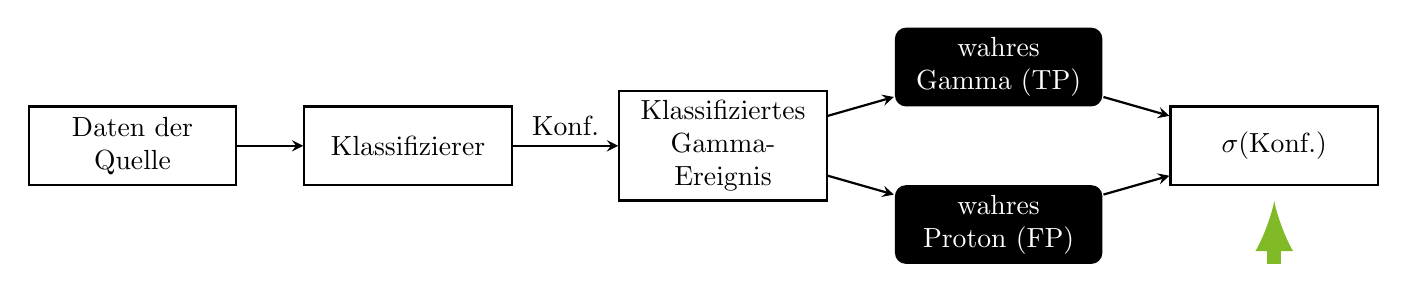
\begin{tikzpicture}[node distance=3.5cm]
  \node (RAW)  [NormalBox] {Daten der Quelle};
  \node (CLAS) [NormalBox, right of=RAW] {Klassifizierer};
  \node (PRED) [NormalBox, right of=CLAS, xshift=0.5cm] {Klassifiziertes Gamma-Ereignis};
  \node (RGAM) [AlternBox, right of=PRED, yshift=1cm] {wahres Gamma (TP)};
  \node (RPRO) [AlternBox, right of=PRED, yshift=-1cm] {wahres Proton (FP)};
  \node (SIGM) [NormalBox, right of=RGAM, yshift=-1cm] {$\sigma$(Konf.)};

  \draw [normalArrow] (RAW) -- (CLAS);
  \draw [normalArrow] (CLAS) -- node[anchor=south] {Konf.} (PRED);
  \draw [normalArrow] (PRED) -- (RGAM);
  \draw [normalArrow] (PRED) -- (RPRO);
  \draw [normalArrow] (RGAM) -- (SIGM);
  \draw [normalArrow] (RPRO) -- (SIGM);
  \draw [printerArrow] ($(SIGM)+(0,-1.5)$) -- ($(SIGM)+(0,-.7)$);

\end{tikzpicture}
\end{document}
